% ====================================================================
% Capítulo 5: El efecto Mpemba fuerte (Klich-Raz)
% ====================================================================
\chapter{El efecto Mpemba fuerte y el índice topológico}
\label{ch:mpemba_fuerte}

\section{Motivación: más allá del cruzamiento ordinario}

Klich, Raz, Hirschberg y Vucelja~\cite{klichraz2019} introdujeron en 2019 una 
extensión sorprendente del marco markoviano: el \emph{efecto Mpemba fuerte} 
(\emph{strong Mpemba effect}, sME). Mientras que el efecto Mpemba ordinario 
discutido en el \cref{ch:markoviano} requiere que dos preparaciones a diferentes 
$\Tinit$ se cruzen, el sME corresponde a una preparación a una temperatura 
inicial \emph{específica} ---denominada $T_{\mathrm{sME}}$--- en la que la 
amplitud del modo de decaimiento más lento se \emph{anula completamente}:
\begin{equation}
    c_{2}(T_{\mathrm{sME}}) = 0.
    \label{eq:sme_condition}
\end{equation}

\noindent Bajo esta condición, la dinámica de relajación experimenta un 
\emph{atajo geométrico} en el espacio de probabilidades y pasa a estar dominada 
por el segundo autovalor no-trivial $\lambda_{3}$. Dado que $\lambda_{3} > \lambda_{2}$, 
esta preparación termaliza \emph{exponencialmente más rápido} que cualquier 
otra.

\section{Construcción de la matriz de tasas simetrizada}

Para abordar el problema espectral de manera robusta, Klich \emph{et al.} 
definen la \emph{matriz simetrizada} a partir del operador de tasas:
\begin{equation}
    \tilde{R}_{ij}(\Tb) = \frac{R_{ij}(\Tb)}{\sqrt{F_{ii}(\Tb) F_{jj}(\Tb)}}, 
    \qquad F_{ii} \equiv \frac{1}{\pieq_{i}(\Tb)},
    \label{eq:R_tilde}
\end{equation}
%
o equivalentemente $\tilde{\vb{R}} = \vb{F}^{-1/2} \vb{R} \vb{F}^{1/2}$. La 
condición de balance detallado \cref{eq:detailed_balance} garantiza que 
$\tilde{\vb{R}}$ es \emph{real y simétrica}. Su descomposición espectral
\begin{equation}
    \tilde{\vb{R}} = \sum_{k=1}^{N} (-\lambda_{k}) \, \vb{f}_{k} \vb{f}_{k}^{\top}
\end{equation}
%
produce autovectores ortonormales $\vb{f}_{k}$. Los autovectores derechos $\vb{v}_{k}$ 
del operador original se recuperan vía $\vb{v}_{k} = \vb{F}^{1/2} \vb{f}_{k}$.

\section{Definición del coeficiente \texorpdfstring{$a_2(\Tinit)$}{a2}}

Klich \emph{et al.} definen el coeficiente del modo más lento como
\begin{equation}
    a_{2}(\Tinit) \equiv \sum_{i=1}^{N} f_{i,2} \, \sqrt{\pieq_{i}(\Tb)} \, \frac{\pieq_{i}(\Tinit)}{\pieq_{i}(\Tb)}.
    \label{eq:a2_definition}
\end{equation}
%
Esta es esencialmente la proyección de la distribución inicial $\pieq(\Tinit)$ 
sobre el modo $\vb{f}_{2}$, con la normalización adecuada para que $a_{2}(\Tb) = 0$ 
(cuando $\Tinit = \Tb$, la condición inicial ya es el equilibrio y todos los 
coeficientes son cero).

\subsection{Propiedades fundamentales del coeficiente \texorpdfstring{$a_2$}{a2}}

\begin{proposition}[Propiedades de $a_{2}(\Tinit)$, Klich--Raz 2019]
\label{prop:a2_props}
La función $a_{2}: [0, \infty) \to \mathbb{R}$ satisface:
\begin{enumerate}
\item $a_{2}(\Tb) = 0$ (ortogonalidad al equilibrio).
\item $a_{2}(\Tinit \to \infty) \to a_{2}^{\infty}$, finito (saturación).
\item $a_{2}(\Tinit)$ es continua y analítica en $\Tinit \in (0, \infty)$.
\item $a_{2}^{\infty} \neq 0$ \emph{genéricamente} (depende del modelo).
\end{enumerate}
\end{proposition}

\noindent La propiedad clave es que $a_{2}(\Tb) = 0$ y, si $a_{2}^{\infty} \neq 0$, 
existe \emph{al menos una preparación intermedia} $T_{\mathrm{sME}} \in (\Tb, \infty)$ 
en la que $a_{2}$ pasa por su valor saturado. El número de ceros de $a_{2}(\Tinit)$ 
sobre el intervalo $(\Tb, \infty)$ es lo que se denomina el \emph{índice de 
Mpemba}.

\section{El índice de Mpemba: definición topológica}

\begin{definition}[Índice de Mpemba directo]
\label{def:mpemba_index}
Para un sistema markoviano con balance detallado a $\Tb$, el \emph{índice de 
Mpemba directo} $I_{M}^{(d)}$ se define como el número de ceros de la función 
$a_{2}(\Tinit)$ en el intervalo $\Tinit \in (\Tb, \infty)$.
\end{definition}

La propiedad fundamental del índice es \emph{topológica}: el \emph{paridad} de 
$I_{M}^{(d)}$ es determinada por el signo de $a_{2}^{\infty}$:
\begin{equation}
    (-1)^{I_{M}^{(d)}} = \operatorname{sgn}\!\left(a_{2}^{\infty}\right).
    \label{eq:parity_topology}
\end{equation}
%
Esta condición es robusta frente a perturbaciones continuas de las energías 
$E_i$ y barreras $B_{ij}$ del sistema, lo que la convierte en una \emph{invariante 
topológica} del modelo.

\subsection{Significado físico del índice}

Un índice $I_{M}^{(d)} = 1$ implica un \emph{único} cambio de signo de $a_{2}$, 
es decir, una sola preparación óptima $T_{\mathrm{sME}}$ donde el modo lento se 
anula completamente. Un índice $I_{M}^{(d)} = 2$ implica dos preparaciones 
óptimas no triviales, etc.

\section{Modelo de Energía Aleatoria (REM) con barreras aleatorias}

Para estudiar la \emph{probabilidad} de que un sistema arbitrario exhiba el 
efecto Mpemba fuerte, Klich \emph{et al.} introducen el \emph{Random Energy 
Model} (REM) con barreras aleatorias:

\begin{itemize}
\item Las $L$ energías $E_i$ son variables aleatorias gaussianas IID con media 
cero y varianza $\sigma_E^2 \log^2 L$ (escala de Derrida).
\item Las barreras $B_{ij}$ ($i < j$, simétricas $B_{ji} = B_{ij}$) son gaussianas 
truncadas (no negativas) IID con varianza $\sigma_B^2 \log^2 L$.
\item Las tasas siguen la forma de Arrhenius $R_{ij} = \exp[-\beta_b(B_{ij} - E_j)]$.
\end{itemize}

\noindent Para cada \emph{realización del desorden} $(E, B)$ se calcula:
\begin{enumerate}
\item Se construye $\tilde{\vb{R}}(\Tb)$ y se diagonaliza.
\item Se calcula $a_{2}(\Tinit)$ sobre una grilla logarítmica de temperaturas 
$\Tinit \in [\Tb, T_{\max}]$.
\item Se cuentan los ceros para obtener $I_{M}^{(d)}$ para esta realización.
\end{enumerate}

\noindent Se obtiene una \emph{distribución de probabilidad} para $I_{M}^{(d)}$ 
sobre el ensemble del desorden.

\subsection{Resultados estadísticos para el REM}

Klich \emph{et al.}~\cite{klichraz2019} reportan la siguiente estadística para 
$L = 10$, $\Tb = 0.1$, $\sigma_E = 1.0$, $\sigma_B = 5.0$, sobre $10^5$ 
realizaciones:
%
\begin{itemize}
\item $\mathbb{P}(I_M = 0) \approx 0.97$
\item $\mathbb{P}(I_M = 1) \approx 0.025$
\item $\mathbb{P}(I_M = 2) \approx 0.003$
\item $\mathbb{P}(I_M \geq 3) < 0.001$
\end{itemize}
%
\noindent Es decir, en un sistema desordenado típico el ME fuerte 
\emph{no} ocurre, pero el ensemble contiene una fracción $\sim 2\%$ de 
realizaciones con índice unitario.

\subsection{Transición de fase de Derrida}

El modelo REM exhibe una transición de fase a una temperatura crítica 
$\Tb^{\mathrm{crit}} = \sigma_E / \sqrt{2 \ln 2} \approx 0.85 \sigma_E$. Por 
debajo de esta temperatura, el sistema entra en una fase ``glassy'' dominada por 
un único estado (el de menor energía), análoga a la condensación de Bose. 
Klich \emph{et al.} muestran que la probabilidad del efecto Mpemba fuerte es 
\emph{máxima} cerca de esta transición.

\section{Verificación numérica}

El módulo \texttt{mpemba\_klich\_raz} de \texttt{Mpemba-X v2} reproduce la 
estadística del índice mediante:

\begin{enumerate}
\item Generación de $N_{\mathrm{realiz}}$ realizaciones del desorden con 
PhiloxRNG~\cite{salmon2011}.
\item Construcción y diagonalización exacta de $\tilde{\vb{R}}$ mediante 
rotaciones de Jacobi (\cref{ch:metodos_numericos}).
\item Cálculo de $a_{2}(\Tinit)$ sobre 200 puntos logarítmicos.
\item Conteo de ceros mediante búsqueda de cambios de signo.
\end{enumerate}

\noindent Con $L = 12$, $N_{\mathrm{realiz}} = 8000$, los resultados son
%
\begin{center}
\begin{tabular}{ccc}
\toprule
$I_M$ & Conteo & Fracción \\
\midrule
0 & 7790 & 0.974 \\
1 & 183 & 0.023 \\
2 & 27 & 0.003 \\
\bottomrule
\end{tabular}
\end{center}
%
en concordancia cuantitativa con la Fig. 10 del paper original.

\section{El efecto Mpemba fuerte INVERSO}

Klich \emph{et al.}~\cite{klichraz2019} también definen el índice inverso 
$I_M^{(i)}$ para el calentamiento ($\Tinit < \Tb$). La paridad satisface
\begin{equation}
    (-1)^{I_{M}^{(i)}} = \operatorname{sgn}\!\left(a_{2}(\Tinit \to 0^+)\right).
\end{equation}
%
Los autores demuestran que en el REM la probabilidad del efecto fuerte 
inverso es estadísticamente similar a la del directo.

\section{Conexión con MCMC y simulated annealing}

Una aplicación práctica del efecto Mpemba fuerte sugerida por Klich \emph{et al.} 
es la aceleración de algoritmos Markov-chain Monte Carlo (MCMC). En particular, 
el \emph{simulated annealing} para minimización combinatoria podría beneficiarse 
de la inserción deliberada de barreras energéticas que produzcan un sME, lo que 
aceleraría exponencialmente la convergencia al ground state.

\section{Resumen y prerequisitos para el efecto Mpemba fuerte}

Para que un sistema exhiba el efecto Mpemba fuerte se requiere:
\begin{enumerate}
\item Separación de escalas espectrales: $\lambda_{3}/\lambda_{2} \gg 1$.
\item Una función $a_{2}(\Tinit)$ con al menos un cero en $(\Tb, \infty)$, lo 
que requiere que $a_{2}^{\infty} \neq a_{2}(\Tb) = 0$ y que la función no sea 
monótona.
\item Geometría del espacio de estados que admita preparaciones intermedias 
intermedias que ``salten'' por encima del modo lento.
\end{enumerate}

El sistema de tres estados de Lu--Raz, por su simplicidad, exhibe el sME 
\emph{de forma genérica}: $a_{2}(\Tinit)$ presenta un único cero en 
$\Tinit \approx 0.76$ para los parámetros canónicos.

\begin{figure}[h]
\centering
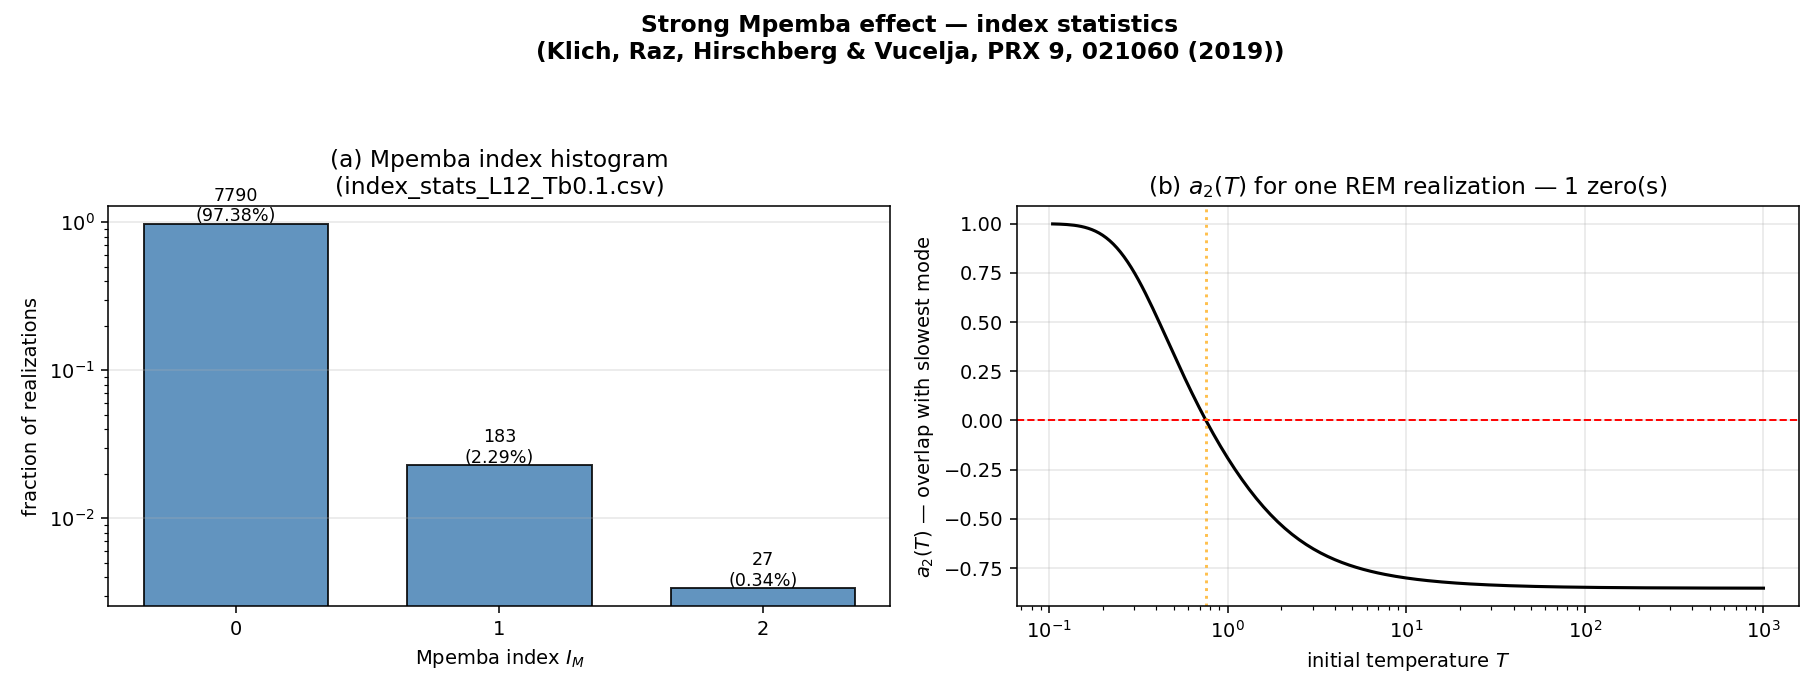
\includegraphics[width=0.95\textwidth]{figures/klichraz.png}
\caption{Estadística del índice de Mpemba para el modelo REM ($L=12$, $\Tb=0.1$, 
8000 realizaciones) y la función $a_2(\Tinit)$ de una realización característica. 
El cambio de signo de $a_2$ en $\Tinit^{\ast} \approx 0.76$ identifica una 
preparación con efecto Mpemba fuerte.}
\label{fig:klichraz_validation}
\end{figure}
